% !TeX root = ../thuthesis-example.tex

\chapter{Platform application}

The platform has already been used for research in a VR-IoT environment.
For their course projects, students in the Autumn 2020 HCIT course were required to research an interaction method in a specific Smart environment simulated in Virtual reality. Each team was given an Oculus Quest 2 VR headset for testing their demos. At the time of the coursework development, students had access to the previous version of the NUIX-Studio platform based on the fourth prototype. As mentioned in chapter 6, this prototype could not convenient create devices, facilitate simultaneous work, or integrate most IoT devices from the real world. However, the platform provided tools for interaction with virtual IoT devices. Students integrated the platform into their projects, which were written in Unity, by adding Widgets such as Sight Sensor, gesture recognition, video streaming, and virtual controls. They also tested various hypotheses for interacting with devices in Virtual reality. As a result, the platform helped to achieve important results in students' course projects. 

Next, selected course projects will be presented. For each of the projects, the research subject is specified first, followed by sections on the experiment its results.

\section{Autumn Semester Student Course Projects}

\subsection{A comparative study of equipment positioning based on spatial location and sound feedback}

Team members:
\begin{enumerate}
    \item Liang Wenjie
    \item Wang Zixuan
    \item Sun Shikun
    \item Saito Fumiki
\end{enumerate}

\subsubsection{Research subject}

Many people encounter the situation of not being able to find their mobile phones before going outside. Usually, people can only determine the approximate location of their smartphone, and it is difficult to specify the exact location of the device quickly. 
In some situations, when preparing for an exam, traveling, etc., people need to search for multiple devices simultaneously. Searching for a single device at once may not be effective.
This team introduced influencing factors such as spatial location and voice feedback to design a more convenient interaction method for device positioning in Smart home scenarios. 

\subsubsection{Experiment}
The team implemented two single device positioning methods:
\begin{enumerate}
    \item Baseline scheme: basic positioning of the device based on sound feedback;
    \item Team solution: positioning of the device based on spatial location and sound changes: when the angle between the user's current orientation and the user-device connection direction is smaller, the volume is louder.
\end{enumerate}

Nine students participated in the experiment. Each time, one device was placed in the virtual NUIX-Studio Smart home environment. The experiment participants were asked to find the device by using each of the two positioning methods (Figure~\ref{fig:Project1-1-figure}).

\begin{figure}
  \centering
  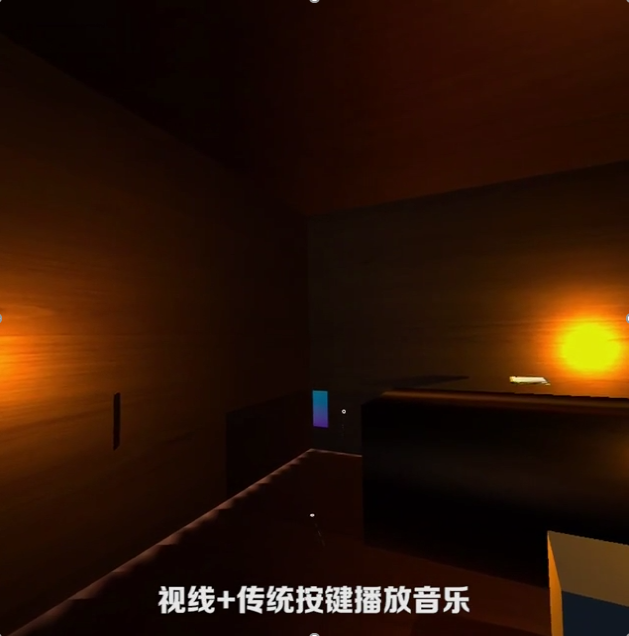
\includegraphics[width=0.6\linewidth]{figures/Project_1-1.png}
  \caption{Screenshot of the project demo.}
  \label{fig:Project1-1-figure}
\end{figure}

In the second experiment, multiple device positioning methods were tested:
\begin{enumerate}
    \item Baseline scheme: basic positioning of the devices based on sound feedback;
    \item Team solution: Each object reports its spatial position by voice commands. If it is in the same room as the user, the position relative to the user will be reported. If the current object is closer to the previous object, the position relative to the previous object is reported. \end{enumerate}

Ten students participated in the second experiment. Each time they were asked to search for the devices using the baseline and team solutions and then give a score to each of the solutions based on the interaction efficiency, learning cost, fatigue level, and user experience. 

\subsubsection{Results}

For the first experiment, students have collected the following results:
\begin{enumerate}
    \item The average time spent by the test group is generally about 15s slower than the baseline (Figure~\ref{fig:Project1-figure});
    \item The test group's maximum time is about 110s, which is much slower than the baseline. The test group's time was affected by the two factors of object distance and corresponding angle.
\end{enumerate}

\begin{figure}
  \centering
  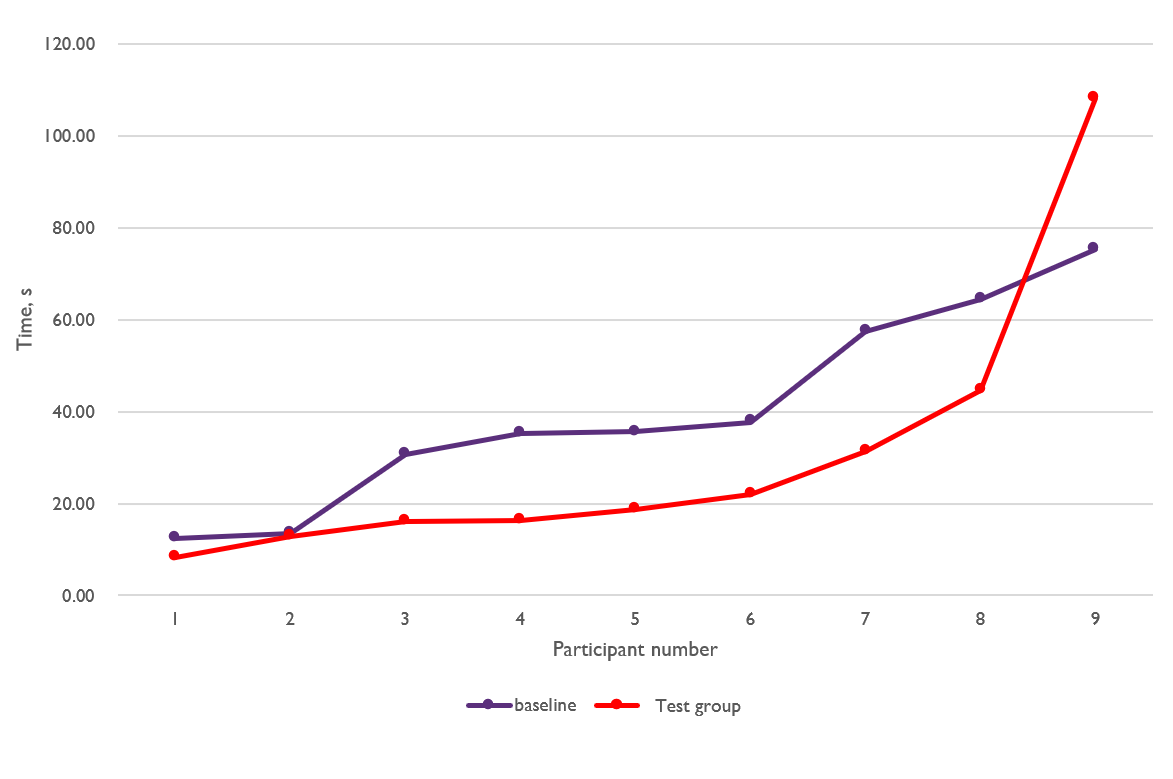
\includegraphics[width=0.9\linewidth]{figures/Project_1.png}
  \caption{Statistics and analysis of user experiment results: objective comparison experiment (single single device positioning time).}
  \label{fig:Project1-figure}
\end{figure}

In the second experiment, most users mentioned that interaction efficiency had been significantly improved using the Team solution. However, there is little difference in terms of learning costs and fatigue levels because, for finding objects, processing the sound information is not as direct as using visual information. 

\subsection{Trigger mechanism of device switching in the Smart home scenario}

Team members:
\begin{enumerate}
    \item Huang Yanwen 
    \item Liu Wei 
    \item Liu Niqi 
    \item Zhang Xueying 
\end{enumerate}

\subsubsection{Research subject}

People often use multiple devices with similar functionality. For example, TVs, computers, and mobile phones all have screens. The traditional methods of switching a certain display content from one device to another include using buttons, remote controls, etc. This team developed novel triggering methods to provide users a more natural, comfortable experience.

The first method is based on using the Sight sensor Widget. When the user's line of sight intersects with a specific display for a certain time, the device is selected.

The second method is based on using the Location Widget. The device activation sensor triggers when the user is a certain distance from the screen.

The third method is based on the gesture recognition Widget. Users use ``grab'' and ``throw'' gestures to move content from one display to another.
 
The fourth method is based on button Widgets, which users can press to switch between the displays.

\subsubsection{Experiment}

The team members conducted a comparison and analysis of the developed trigger methods through several evaluation experiments.(Figure~\ref{fig:Project2-figure}).

\begin{figure}
  \centering
  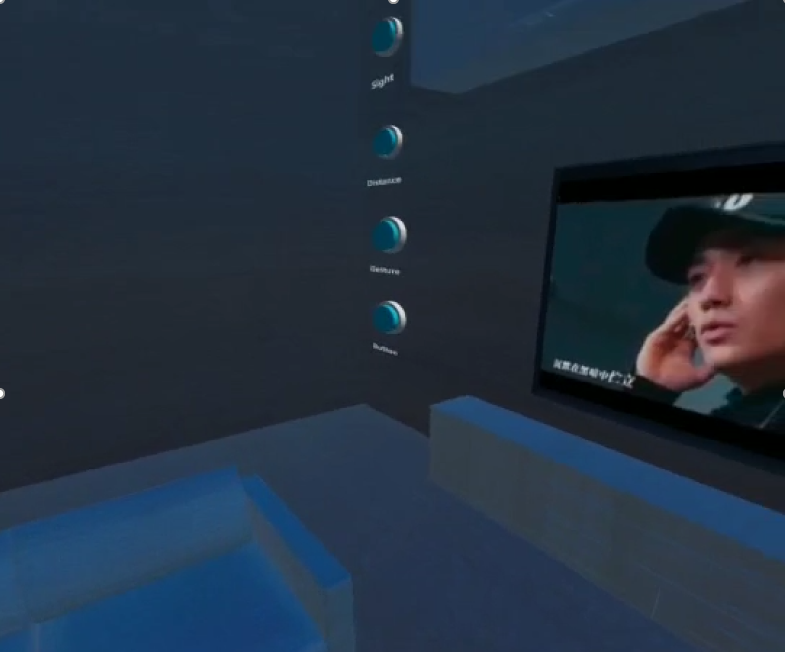
\includegraphics[width=0.6\linewidth]{figures/Project_2.png}
  \caption{Demo of the project.}
  \label{fig:Project2-figure}
\end{figure}

\subsubsection{Results}

The easiest method to use is sight-based interaction(Figure~\ref{fig:Project10-figure}), while the gesture-based method provides the most natural user experience, sense of control and user satisfaction.

The failure rate of gesture recognition is 5\%, primarily because of the instability of the device's hand recognition.
The user's low evaluation of button control is mainly due to the lack of tactile feedback in VR and unstable hand recognition, causing the button to fail to be triggered when pressed or double-clicked.

The basis for fast device switching is the remote interconnection of multiple devices. Although the current Smart home environments have not fully achieved this goal, the team believes this is an inevitable trend in the future.\footnote{Using the final prototype of the NUIX-Studio, researchers can implement remote interconnection between real and virtual devices}


\begin{figure}
  \centering
  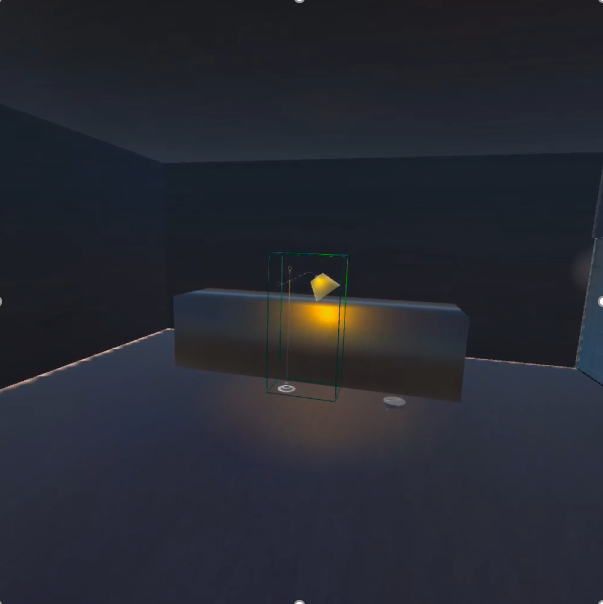
\includegraphics[width=0.6\linewidth]{figures/Project_10.png}
  \caption{Demo of another team project. By exploring the meaning of sight awakening, students Wei Tong, Chen Bohan, Lu Mengying and Zou Tianyuan developed a sight interaction method based on statistical models. }
  \label{fig:Project10-figure}
\end{figure}

\subsection{Smart gloves - New interactive devices in smart medical scenarios}

This project is not especially novel, but it demonstrates how the NUIX-Studio platform can be easily integrated into a specific Smart environment.

Team members:
\begin{enumerate}
    \item Deng Bowen 
    \item Niu Haoyu
    \item Wang Shijie 
    \item Zhou Huanhai 
\end{enumerate}


\subsubsection{Research subject}

In hospitals, patients are often restricted in their activities and cannot easily complete operations such as turning on and off the lights and adjusting beds by themselves.

This team designed a new type of interaction method based on smart glove usage, helping patients interact with devices through gestures and hand movements. Smart gloves can be represented in VR by hand recognition technology.

\subsubsection{Experiment}

The team has added support for several gestures into the gesture recognition Widget to control the objects inside a virtual hospital environment (Figure~\ref{fig:Project4-figure}).
Next, the students performed a user study to evaluate four parameters: ease of use, interaction efficiency, fatigue and practicality. 

\begin{figure}
  \centering
  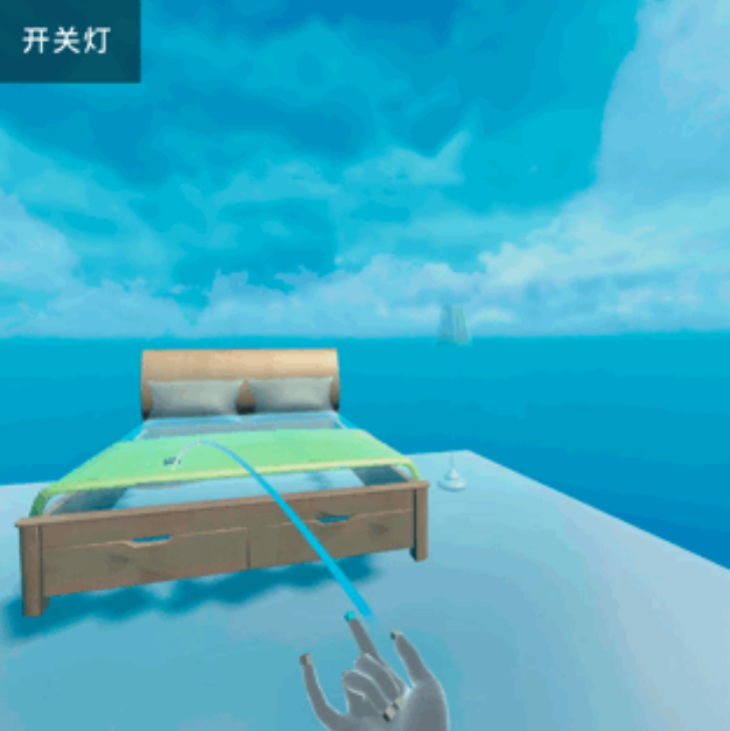
\includegraphics[width=0.6\linewidth]{figures/Project_4.png}
  \caption{One of the gestures developed. Use gesture similar to ‘Spider-Man’ (right middle finger and ring finger) to trigger the light switch.}
  \label{fig:Project4-figure}
\end{figure}

\subsubsection{Results}
The users found the demo easy to use, efficient, and practical, but most felt moderately tired after the 5-minute experiment.

\subsection{Research on Feedforward of Home Appliance Control Based on MRTK}

Team members:
\begin{enumerate}
    \item Li Ziang
    \item Li Ao
    \item Sui Weiyi
\end{enumerate}

\subsubsection{Research subject}

It is difficult for users to remember the mapping relationship between gestures and home appliance functions.
The solution is to add visual feed-forward and trigger prompts by using a Sight Widget.

\subsubsection{Experiment}

Participants used the Smart home environment and a Gesture recognition Widget from NUIX-Studio to test the demo's ease of learning (Figure~\ref{fig:Project7-figure}). The users needed to complete multiple tasks within 5 minutes without any prior knowledge.
Next, completion rate and user ratings were collected and analyzed.

\begin{figure}
  \centering
  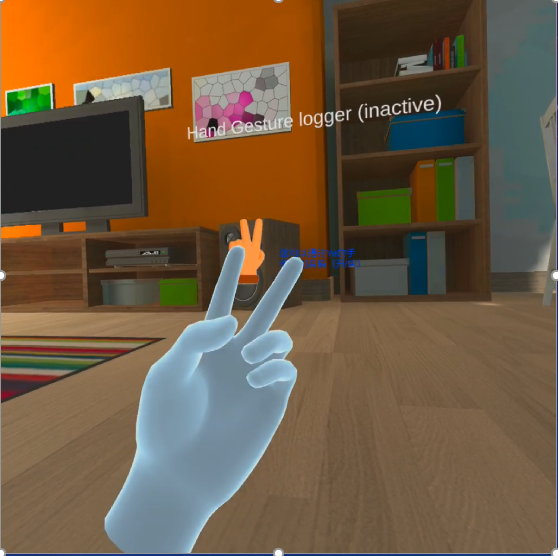
\includegraphics[width=0.6\linewidth]{figures/Project_7.png}
  \caption{Combine sight detection and gesture recognition
When the fixation time exceeds the threshold, a prompt will pop up.}
  \label{fig:Project7-figure}
\end{figure}

\subsubsection{Results}

Average score: 4.14 points (out of 5 points)
Average task completion rate: 65.29\%

\subsection{Gesture laser pointer}

Team members:
\begin{enumerate}
    \item Wang Haoyu
    \item Zhang Zeyuan 
    \item Zhang Zizhao
\end{enumerate}


\subsubsection{Research subject}
Teachers can use computers and writing pads at the podium to mark content conveniently, but they are far from the students, making the interaction between them weak.
When teachers are standing next to the desks, the interaction between students and teachers becomes closer. However, it is difficult for the teachers to mark content effectively without the computer and writing board.
The team wanted to test if the laser pointer's function could be extended so that teachers could effectively mark content.

This team has developed a gesture laser pointer based on the gesture recognition Widget that does not need to be held in one's hand.
The developed tool can perform the functions of lighting, drawing rectangles, drawing circles and erasing content.

\subsubsection{Experiment}

The participants were asked to draw rectangles and circles around characters of different sizes (Figure~\ref{fig:Project9-figure}). 

\begin{figure}
  \centering
  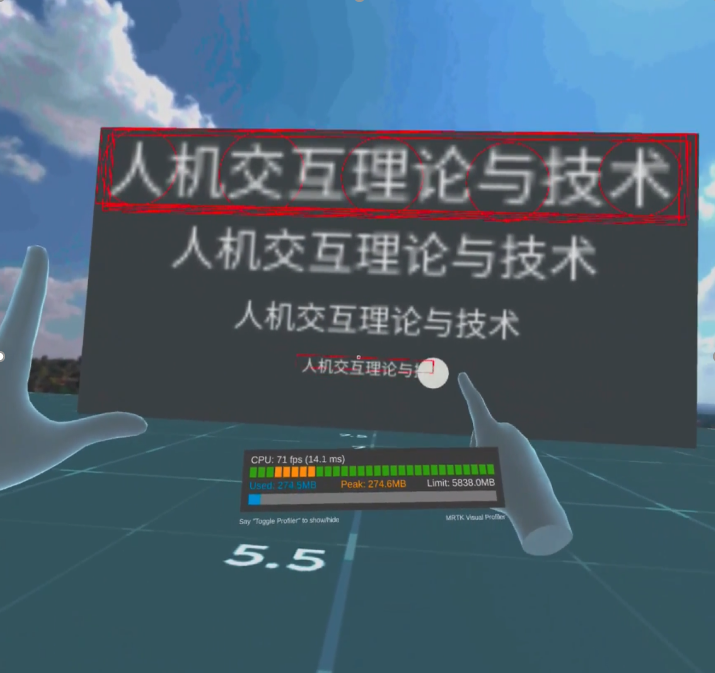
\includegraphics[width=0.6\linewidth]{figures/Project_9.png}
  \caption{Demo of the Gesture laser pointer experiment.}
  \label{fig:Project9-figure}
\end{figure}


\subsubsection{Results}

The average time to perform an experimental task varied from 3 to 5 seconds. The accuracy of drawing varied from 87.5\% to 97.5\%.

The average user satisfaction score was 8.46 points out of 10 points.

Overall the team has implemented a unique instrument, which can be added to NUIX-Studio as a Widget for a Smart classroom environment.

\subsection{FloorUI—home control system based on interactive ground}

Team members:
\begin{enumerate}
    \item Zhang Xiaoyu
    \item Zhu Yihao
    \item Xie Yuqing
    \item Zhang Yizhuo
\end{enumerate}


\subsubsection{Research subject}

In this project, the students explored the operation of equipment in a hands-free manner by setting a wake-up UI interface on the floor (Figure~\ref{fig:Project11-figure}). 

\begin{figure}
  \centering
  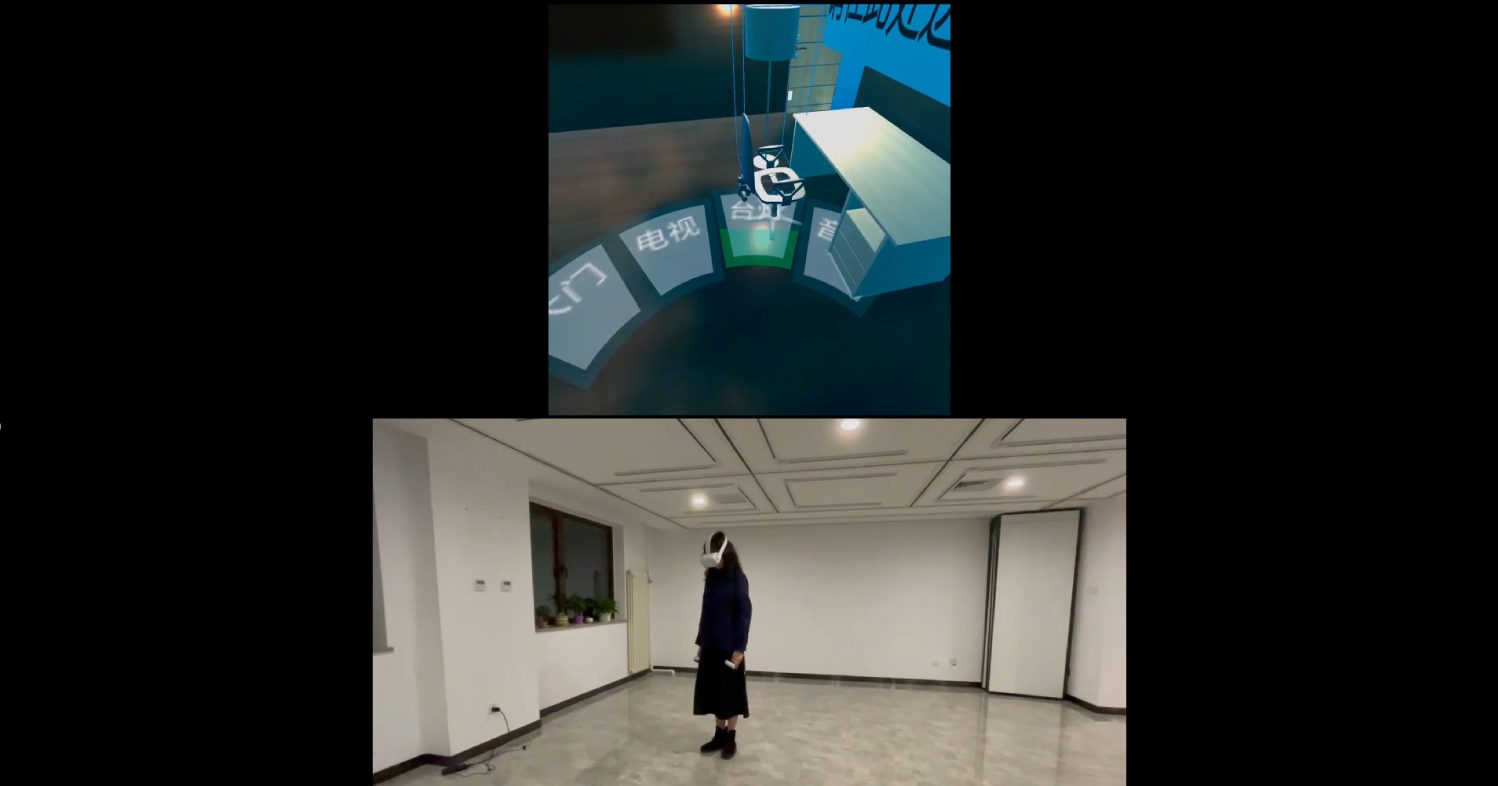
\includegraphics[width=0.9\linewidth]{figures/Project_11.png}
  \caption{Demo of the experiment.}
  \label{fig:Project11-figure}
\end{figure}

\subsubsection{Experiment}

Two different ways of interacting with the UI were tested:
\begin{enumerate}
    \item Gaze interaction. The UI element is selected by the user's gaze point. Each of the buttons can be pressed by triggering a corresponding Sight sensor Widget.
    \item Body interaction. The UI element is selected by the user's feet positioning (Figure~\ref{fig:Project11_1-figure}). By streaming the camera from the phone to Unity (Figure~\ref{fig:VideoStreamingWidget-figure}), the virtual location of the user's feet is calculated.
\end{enumerate}


\begin{figure}
  \centering
  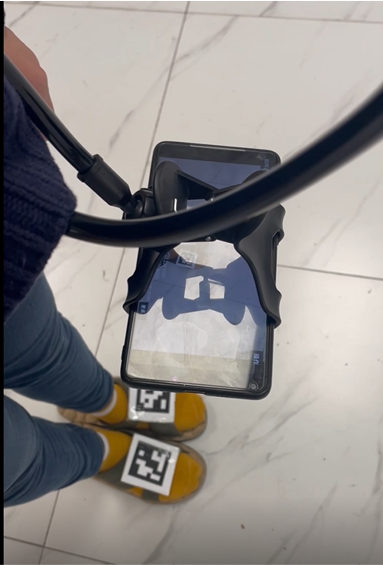
\includegraphics[width=0.6\linewidth]{figures/Project_11_1.png}
  \caption{Get the feet position by placing a QR code on the user's shoes.}
  \label{fig:Project11_1-figure}
\end{figure}


\begin{figure}
  \centering
  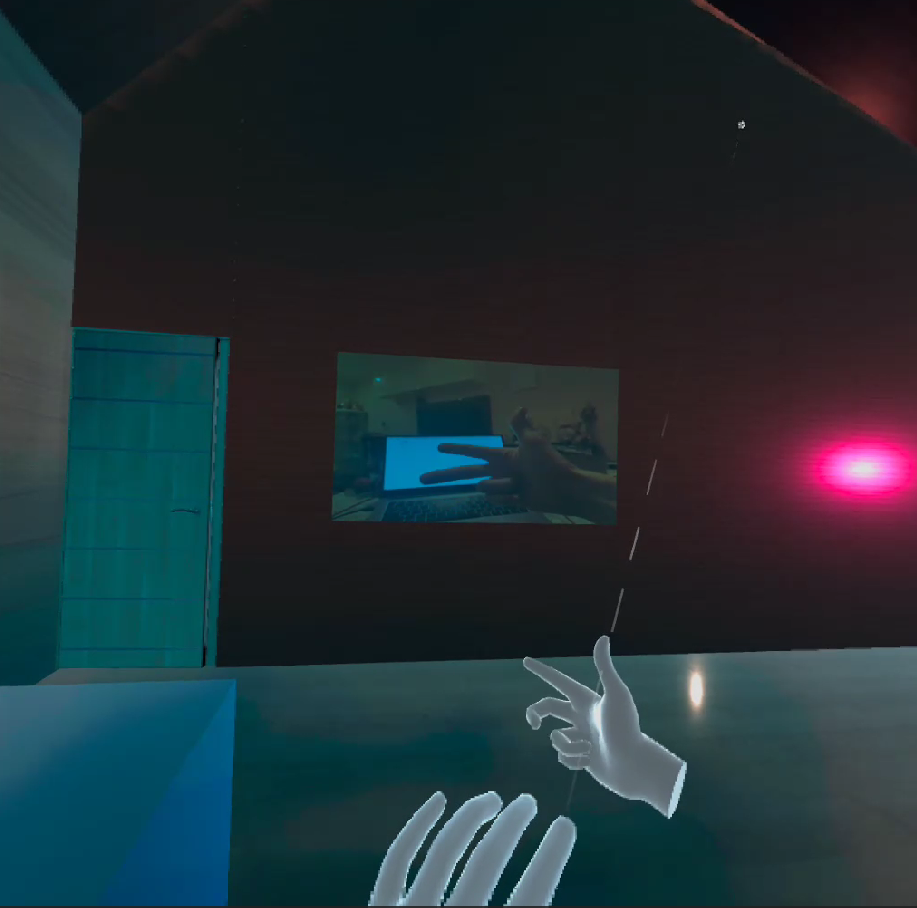
\includegraphics[width=0.6\linewidth]{figures/VideoStreamingWidget.png}
  \caption{Video Streaming widget of the NUIX-Studio used by students.}
  \label{fig:VideoStreamingWidget-figure}
\end{figure}


There were 4 steps in the experiment:
\begin{enumerate}
    \item Getting familiar with the virtual Environment;
    \item Testing gaze interaction (2 rounds, rest between rounds);
    \item Testing body interaction (1 round);
    \item Completion of the questionnaire.
\end{enumerate}

\subsubsection{Results}

By analyzing the time the user took to wake up the UI and make a choice, the following results were obtained:
\begin{enumerate}
    \item Both waking up the UI and making a choice are easy to learn for users;
    \item After the user is fully familiar with the two interaction methods and scenarios, it takes 8.3s and 9.5s on average to perform the selection using gaze and body interactions, respectively (this includes the 3.5s required to wake up the UI and confirm the choice). The body interaction method is relatively fast and convenient;
    \item The users succeeded in a total of 101 UI wake-up operations, and there was no false triggering of UI wake-up. Among the 70 sight selections, there were 5 cases in which the user intended to confirm the option but did not succeed, but there was no case where the wrong option was confirmed. 
    \item Most participants agreed that line-of-sight interaction is more natural. The team believes that this may be caused by the discomfort of wearing VR Headsets.
\end{enumerate}

\section{Spring Semester Student Course Projects}

Students of the Spring 2021 HCIT course introduced examples of how to use IoT devices for messaging, listening to music, reading news and friends' news feed, watching videos and creating memos in different environments. Thus, it is necessary to provide students with a more detailed tutorial on how to run the platform and add new examples of interaction with Widgets. In addition, the author proposes to create a way to distribute the  Widgets between the teams so that students could focus more on the HCI aspects and User study. 

Several teams have already implemented prototypes of their projects. In comparison to the previous semester, it takes less time for the students to understand the concepts of Items and Widgets and to build their own Smart devices from the functional blocks, not only because of better documentation and clearer structure but also because of the available video tutorials on using the NUIX-Studio App. According to the feedback from the students of the course, the main difficulty is to understand the concepts of Unity and how to write code in C\# language. Users will only need to run NUIX-Studio App for developing new IoT devices without writing any code in Unity software in the next prototypes.